\chapter{Implementace}

Tato kapitola popisuje implementaci celé aplikace nad geografickými i negeografickými daty. Aplikační architektura je modulární a odděluje prezentační vrstvu, doménovou logiku optimalizace, routovací integrace (OpenRouteService/OSRM) a vrstvu I/O.

Z hlediska odpovědnosti modulů je systém rozdělen následovně:
\begin{itemize}
    \item \texttt{tsp\_solver/ui} -- uživatelské rozhraní (sidebar, mapa, pravý panel s trasou),
    \item \texttt{tsp\_solver/core} -- orchestrace výpočtu a běh optimalizačních algoritmů,
    \item \texttt{tsp\_solver/routing} -- tvorba trasových matic, volání ORS/OSRM a zpracování odpovědí,
    \item \texttt{tsp\_solver/io} -- import/export instancí ve formátech TSPLIB (GEO/EUC\_2D) a GPX,
    \item \texttt{tsp\_solver/state} -- centrální aplikační stav a perzistence nastavení.
\end{itemize}

Jádrem výpočtu je třída \texttt{TSPManager}, která zajišťuje celý výpočetní pipeline: validaci vstupu, volbu efektivní metriky, sestavení matice vzdáleností/časů, spuštění zvoleného solveru, výpočet agregované hodnoty trasy a následné vygenerování geometrie pro mapovou vizualizaci.

\lstinputlisting[
    language=Python,
    basicstyle=\footnotesize\ttfamily,
    columns=fullflexible,
    breaklines=true,
    tabsize=2,
    caption={Řízení výpočtu trasy v \texttt{TSPManager}},
    label=src:tspmanager_pipeline
]{SourceCodes/tspmanager_pipeline.py}

Jednotné volání konkrétních solverů obstarává \texttt{OptimizationEngine}. Podle zvoleného klíče vybere implementační funkci a předá jí pouze argumenty, které signatura této funkce přijímá.

\lstinputlisting[
    language=Python,
    basicstyle=\footnotesize\ttfamily,
    columns=fullflexible,
    breaklines=true,
    tabsize=2,
    caption={Mapování solverů a metoda \texttt{run} v \texttt{OptimizationEngine}},
    label=src:optimization_engine_dispatch
]{SourceCodes/optimization_engine_dispatch.py}

\section{Implementace generátoru instancí}
Generování instancí je v implementaci řešeno kombinací interaktivního a dávkového přístupu. Historicky byl v návrhu samostatný \texttt{InstanceGenerator}, ale výsledná implementace tuto funkcionalitu rozpouští do UI a I/O strategie, což se v praxi ukázalo jako jednodušší na údržbu.

\subsection{Vstupní data a model reprezentace bodů}
Interně jsou body reprezentovány jako dvojice \texttt{(x, y)}; u geografického režimu jde o \texttt{(lat, lon)}, u eukleidovského režimu o \texttt{(x, y)} v rovině. Aplikační stav ukládá:
\begin{itemize}
    \item seznam bodů,
    \item volitelné textové popisky bodů,
    \item příznak \texttt{is\_geographic},
    \item vypočtenou trasu a metadata výsledku.
\end{itemize}

Body lze získat:
\begin{enumerate}
    \item klikáním do mapy (geografický režim),
    \item geokódovacím vyhledáním lokality přes ORS autocomplete,
    \item importem \texttt{.tsp} nebo \texttt{.gpx}.
\end{enumerate}

Tím je dosaženo toho, že stejná výpočetní část aplikace pracuje jak s reálnými geografickými instancemi, tak se syntetickými rovinými daty.

\subsection{Funkce pro výpočet vzdáleností mezi všemi body pomocí mapových API}
Výpočet matic je v třídě \texttt{DistanceMatrixBuilder}. Implementace podporuje dva typy metrik:
\begin{itemize}
    \item \textbf{bodové metriky} (Haversine, EUC\_2D, Manhattan, Chebyshev) -- matice je sestavena lokálním výpočtem dvojic bodů
    \item \textbf{trasové metriky} (\texttt{routing\_dist}, \texttt{routing\_time}) -- matice se získává přes ORS Matrix API, případně fallback na lokální OSRM Table API
\end{itemize}

Při požadavku na trasovou metriku se nejdříve z konfigurace ověří dostupnost ORS API klíče. Pokud je klíč přítomen, systém volá endpoint \texttt{/v2/matrix/\{profile\}}. Kvůli limitu ORS na počet párů zdroj--cíl (\texttt{ORS\_MATRIX\_MAX\_PAIRS = 2500}) je implementováno blokové dělení matice na submatice. Výsledná matice se skládá blokově a je poté dostupná pro zbytek pipeline.

Pokud ORS volání selže nebo není API klíč nastaven, a je povolen fallback, použije se lokální OSRM (\texttt{http://localhost:5000}) s endpointem \texttt{/table/v1/\{profile\}/}. Teprve při selhání obou trasových backendů se výpočet degraduje na Haversine metriku.

\lstinputlisting[
    language=Python,
    basicstyle=\footnotesize\ttfamily,
    columns=fullflexible,
    breaklines=true,
    tabsize=2,
    caption={Větev \texttt{ROUTING\_DIST} ve \texttt{DistanceMatrixBuilder.build}},
    label=src:distance_matrix_routing_fallback
]{SourceCodes/distance_matrix_routing_fallback.py}

\subsection{Ukládání matice vzdáleností}
Matice je uložena jako dvourozměrné pole \texttt{list[list[float]]}. Hodnoty na diagonále jsou nulové, nedostupné trasy jsou reprezentovány hodnotou \texttt{inf}. Tato reprezentace je kompatibilní se všemi implementovanými metodami a umožňuje jednotné API optimalizačního jádra.

Matice se aktuálně počítá při každém běhu výpočtu a explicitně se neukládá do samostatného perzistentního souboru. Perzistují se vstupní body (a případně route body v GPX), což je zvoleno záměrně: odstraňuje to riziko nekonzistence mezi geometrií bodů, profilem routingu a uloženou maticí.

\section{Generování reálných a syntetických instancí}
Systém podporuje dva režimy vytvářeníinstancí: geografický (reálné lokality) a negeografický (syntetické rovinné body).

\subsection{Generování podle reálných měst}
Reálné instance jsou typicky tvořeny:
\begin{itemize}
    \item vyhledáním měst přes ORS geokódování (\texttt{MapSearchBar}),
    \item importem existujících TSPLIB GEO instancí,
    \item importem GPX bodů.
\end{itemize}

Každý vybraný výsledek u mapového vyhledávání obsahuje souřadnice i textový label, který je při vložení bodu uložen do stavu a zároveň do perzistentní geocode cache.

U GEO TSPLIB importu je implementována důležitá kompatibilitní logika: pokud soubor neobsahuje aplikační značku \texttt{COMMENT: MODERN\_GPS}, parser předpokládá historický TSPLIB GEO formát \texttt{DDD.MM} a převádí jej na desetinné stupně. To umožňuje korektní načtení referenčních knihovních instancí bez ručního zásahu.

\subsection{Náhodné generování souřadnic (syntetické instance)}
Syntetická data jsou reprezentována jako \texttt{EUC\_2D} instance. Prakticky vznikají dvěma cestami:
\begin{enumerate}
    \item importem externě vytvořených \texttt{EUC\_2D} TSPLIB souborů,
    \item interaktivním skládáním bodů v negeografickém režimu.
\end{enumerate}

Pro zobrazení v mapové komponentě je u negeografických bodů použita normalizace do vizuálního souřadného prostoru. Tím je zajištěno, že i data bez geodetického významu lze přehledně vykreslit nad Leaflet scénou, aniž by systém předstíral reálné mapové dlaždice.

\subsection{Automatizované generování}
Automatizační vrstva je implementována primárně jako automatizace výpočetního workflow:
\begin{itemize}
    \item volitelný automatický přepočet trasy po přidání/odebrání bodu,
    \item automatické přednačítání detailů trasy (instrukce, elevace) po dokončení výpočtu,
    \item automatické ukládání částí konfigurace do \texttt{QSettings}.
\end{itemize}

Samostatný dávkový generátor syntetických instancí není součástí hlavního běhu aplikace. Jádro aplikace je v importně-exportních funkcích a v interaktivním skládání instancí v grafickém rozhraní.

\section{Optimalizace výkonu a správa zdrojů}
\label{sec:implementace_vykonu}
Implementace řeší výkon ve třech rovinách: algoritmická optimalizace solverů, neblokující běh UI a omezení zbytečných síťových volání.

\subsection{Přechod od návrhu ke kódu}
Výpočet trasy je spouštěn v separátním \texttt{QThread} workeru (\texttt{\_SolveWorker}), aby hlavní UI vlákno zůstalo responzivní. Tento přístup je použit i pro stahování detailních directions dat v pravém panelu.

\texttt{QObject} worker produkuje signály \texttt{finished}/\texttt{failed}, řídící funkce korektně ukončí vlákno a objekty se mažou pomocí \texttt{deleteLater}. Tím se minimalizuje riziko úniku paměti a zároveň je zajištěno, že síťově náročné operace neblokují vykreslování mapy.

\lstinputlisting[
    language=Python,
    basicstyle=\footnotesize\ttfamily,
    columns=fullflexible,
    breaklines=true,
    tabsize=2,
    caption={Spuštění \texttt{QObject} workeru v \texttt{QThread} s ukončením přes \texttt{deleteLater}},
    label=src:sidebar_qthread_worker
]{SourceCodes/sidebar_qthread_worker.py}

\subsection{Algoritmické optimalizace}
Kromě výběru více solverů jsou přímo v kódu implementovány mikrooptimalizace:
\begin{itemize}
    \item optimalizační jádro sjednocuje volání metod NN, 2-opt, 3-opt, ACO, GA, SA, LK, RSO a LKH nad jednotným datovým rozhraním matice
    \item u ACO je předpočtena matice viditelnosti \(\eta^\beta\)
    \item počet mravenců je výchozí hodnotou omezen horní hranicí \texttt{min(n, 20)} pro stabilnější dobu běhu, popřípadě lze načíst předem připravené laděné parametry pro určité velikosti instancí
    \item metrický katalog centralizuje validní metriky dle typu instance a omezuje nevhodné kombinace
\end{itemize}

\subsection{Správa síťových zdrojů}
Síťová vrstva používá timeouty jak u \texttt{requests}, tak u Qt síťového klienta:
\begin{itemize}
    \item matrix volání: timeout 60 s,
    \item directions volání: timeout 45 s,
    \item geocode/reverse geocode volání: transfer timeout 12--15 s.
\end{itemize}

Dále je implementována fronta reverzního geokódování s omezenou paralelou (\texttt{max\_concurrent = 2}), která brání požadavkům při rychlé manipulaci s body na mapě.

\subsection{Zpracování chyb a Rate Limiting mapových služeb}
Současná implementace řeší chyby vícevrstvě:
\begin{enumerate}
    \item kontrola HTTP statusu a validace struktury odpovědi,
    \item fallback ORS \(\rightarrow\) lokální OSRM,
    \item fallback trasové metriky \(\rightarrow\) Haversine (pokud selže síťová vrstva).
\end{enumerate}

Pokud API vrátí neúspěšnou odpověď (včetně scénářů typu HTTP 429), volání je vyhodnoceno jako neúspěšné a aktivuje se fallback větev. V geokódovacích widgetech se při chybě jednoduše skryjí návrhy, aby uživatel neměl nekonzistentní data.

Chování je konzervativní: požadavek buď uspěje, nebo se bez opakování přejde na náhradní zdroj. To je v této etapě vývoje přijatelné díky dostupnosti lokálního OSRM, nicméně pro produkční cloud-only provoz je vhodné doplnit:
\begin{itemize}
    \item řízený retry policy (např. 429/5xx),
    \item exponenciální zvyšování prodlev,
\end{itemize}

Nevalidní odpovědi (chybějící geometry, neočekávaný tvar pole, neparsovatelný JSON) jsou ošetřeny obranou validací a návratem \texttt{None}, což je navázáno na fallback logiku bez pádu aplikace.

\section{Vizualizace}
Vizualizační vrstva kombinuje \texttt{QWebEngineView} (Leaflet mapa) a PyQt overlay prvky.

\subsection{Implementace interaktivní mapy}
Mapa je načtena z lokálního HTML (\texttt{resources/map\_leaflet.html}) a propojena s Pythonem přes \texttt{QWebChannel}. Most \texttt{\_MapBridge} přenáší události:
\begin{itemize}
    \item kliknutí do mapy \(\rightarrow\) přidání bodu,
    \item pravý klik na marker \(\rightarrow\) odstranění bodu.
\end{itemize}

Mapa reaguje na notifikace ze \texttt{AppState} (observer pattern), tj. umí se centrovat, překreslovat body, přepínat mapovou vrstvu, zobrazovat/skrývat indexy bodů a kreslit trasu.

\lstinputlisting[
    language=Python,
    basicstyle=\footnotesize\ttfamily,
    columns=fullflexible,
    breaklines=true,
    tabsize=2,
    caption={Most \texttt{\_MapBridge} a \texttt{QWebChannel} v \texttt{MapViewer}},
    label=src:map_viewer_webchannel
]{SourceCodes/map_viewer_webchannel.py}

\subsection{Zobrazení uzlů a hran}
Uzly jsou vykresleny jako markery. Při postupném přidávání se používá inkrementální přístup, při hromadné změně kompletní překreslení. Tento kompromis snižuje počet operací a přitom zachovává konzistenci.

Hrany trasy se vykreslují buď jako:
\begin{itemize}
    \item přímé úsečky (bodové metriky),
    \item detailní polyline z ORS/OSRM geometrie (trasové metriky).
\end{itemize}

\subsection{Zobrazení nalezeného řešení}
Po solve se do stavu uloží:
\begin{itemize}
    \item polyline trasy,
    \item pořadí zastávek včetně návratu na start,
    \item agregovaná hodnota (km nebo min),
    \item klíč použité metriky.
\end{itemize}

Pravý panel nad mapou rozšiřuje vizualizaci o:
\begin{itemize}
    \item textové navigační instrukce
    \item výškový profil (pokud ORS vrátí 3D geometrii)
    \item odhad spotřeby paliva.
\end{itemize}

Výškový profil je kreslen  widgetem (\texttt{QPainter}), kde osa X reprezentuje kumulativní vzdálenost a osa Y nadmořskou výšku.

% Ukázka uživatelského rozhraní a vykreslené trasy
\begin{figure}[H]
    \centering
    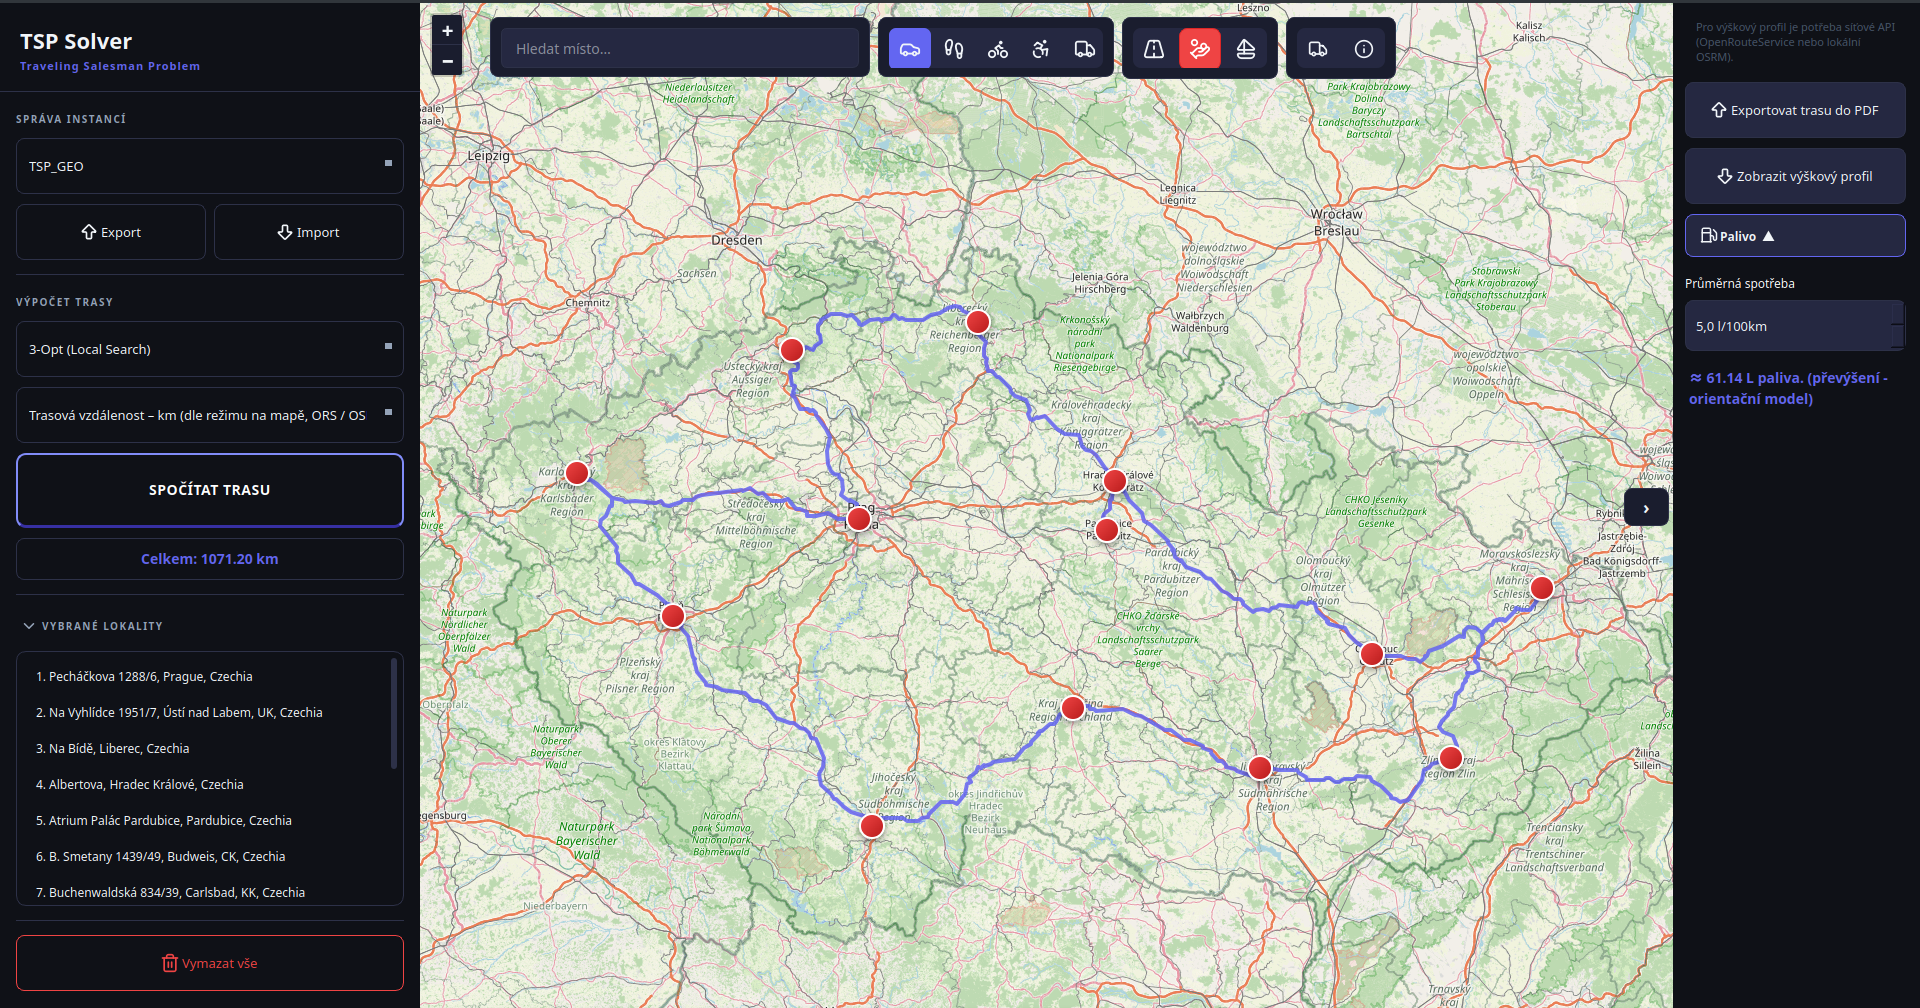
\includegraphics[width=\textwidth]{Figures/ukazka_aplikace.png}
    \caption{Ukázka vizualizační vrstvy aplikace při zobrazení vypočtené trasy}
    \label{fig:ukazka_aplikace}
\end{figure}

\section{Export a kompatibilita}
Exportní vrstva je postavena na strategickém vzoru (\texttt{TspGeoStrategy}, \texttt{TspEuc2DStrategy}, \texttt{GpxStrategy}), což umožňuje přidávat nové formáty bez zásahu do orchestrace.

\subsection{Export do TSPLIB formátu}
TSPLIB export je implementován v následujících variantách:
\begin{itemize}
    \item \texttt{EDGE\_WEIGHT\_TYPE: GEO},
    \item \texttt{EDGE\_WEIGHT\_TYPE: EUC\_2D}.
\end{itemize}

U GEO exportu aplikace zapisuje desetinné stupně a přidává příznak \texttt{COMMENT: MODERN\_GPS\_DIPLOMA}. Tento příznak je klíčový pro zpětnou detekci, zda je nutný historický převod DDD.MM při importu.

Z pohledu kompatibility s externími TSP nástroji je tento přístup robustní. Soubor zůstává validní instancí knihovny TSPLIB, přitom aplikace u vlastních exportů zachovává přesnou informaci o interní interpretaci souřadnic.

\lstinputlisting[
    language=Python,
    basicstyle=\footnotesize\ttfamily,
    columns=fullflexible,
    breaklines=true,
    tabsize=2,
    caption={GEO TSPLIB: značka exportu a převod \texttt{DDD.MM} při importu},
    label=src:tsp_geo_strategy_export_load
]{SourceCodes/tsp_geo_strategy_export_load.py}

\subsection{GPX export/import}
GPX export ukládá waypointy a volitelně i vypočtenou trasu jako \texttt{trkseg}. Pokud uživatel požaduje GPX export bez vypočtené trasy, UI nabídne:
\begin{itemize}
    \item waypoint-only GPX
    \item fallback export do TSP
\end{itemize}

Tato volba je důležitá z hlediska uživatelského očekávání: GPX je primárně navigační formát, zatímco TSP je optimalizační instance.

\subsection{Perzistence konfigurace a provozní kompatibilita}
Aplikační preference jsou uloženy pomocí knihovny \texttt{PyQt6}, konkrétně \texttt{QSettings}:
\begin{itemize}
    \item barevné schéma aplikace (dark/light theme), mapový podklad, jednotky vzdálenosti
    \item ORS klíč, ORS base URL, profil routingu, HGV restrikce
    \item přepínače fallback režimu a automatického přepočtu trasy.
\end{itemize}

ORS klíč a base URL lze zároveň přepsat proměnnými prostředí (\texttt{ORS\_API\_KEY}, \texttt{ORS\_BASE\_URL}), což zvyšuje přenositelnost mezi vývojovým a testovacím prostředím.

Celkově implementace splňuje požadavky na kompatibilitu s referenčními TSPLIB daty, podporuje operace s mapovými službami a zároveň zachovává robustní chování i při částečné nedostupnosti síťových backendů.
\endinput
